\documentclass{beamer}
\usetheme{Boadilla}
\usepackage{tp} 
\newcommand{\iterate}[1]{\textbf{#1}}
\title{Aula 1}
\subtitle{STL}
\author{Maratona de Programação}
\institute{FEI}
\date{\today}
\setbeamertemplate{navigation symbols}{}

\begin{document}
    \begin{frame}
        \titlepage
    \end{frame}
	
	\begin{frame}{O que é STL?}
		\begin{itemize}
			\item Definição
			\begin{itemize}
				\item A \textit{Standard Template Library} (STL) do C++ é um conjunto de templates e funções que fornece implementações comuns de estruturas de dados e algoritmos.
			\end{itemize}

			\item Componentes da STL
            \begin{itemize}
                \item Containers
                \item Algoritmos
                \item Iteradores
                \item Functors
            \end{itemize} 
		\end{itemize}
	\end{frame}

    \begin{frame}{Containers que serão estudados}
       \begin{itemize}
            \item Containers sequenciais
            \begin{itemize}
                \item Vector
            \end{itemize}
            \item Containers associativos
            \begin{itemize}
                \item Set
                \item Map
            \end{itemize}
            \item Containers adaptativos
            \begin{itemize}
                \item Stack
                \item Queue
                \item Priority Queue
            \end{itemize}
       \end{itemize} 
    \end{frame}
    
    \begin{frame}{Vector}
        \begin{itemize}
            \item Resumidamente, \textit{vectors} são containers sequenciais que representam \textit{arrays} dinâmicos.
            \vfill
            \item Diferentemente dos arrays tradicionais, seu tamanho pode ser alterado durante a execução do código, com o armazenamento sendo gerenciado automaticamente pelo container.
            \vfill
            \item Motivação: \href{https://vjudge.net/problem/Aizu-ITP2_1_A}{\textcolor{blue}{\uline{Vector}}}
        \end{itemize}
    \end{frame}

    \begin{frame}{Maneiras de inicializar um vector}
        \lstinputlisting{vector1.cpp} 
    \end{frame}
    
    \begin{frame}{Principais métodos}
        \lstinputlisting{vector2.cpp} 
    \end{frame}

    \begin{frame}{Set}
        \begin{itemize}
            \item São conjuntos que armazenam elementos únicos em alguma ordem de classificação, geralmente crescente.
            \vfill
            \item Geralmente implementados com Árvores Red-Black, que garantem complexidades logarítmicas.
            \vfill
            \item Motivação: \href{https://judge.beecrowd.com/pt/problems/view/2653}{\textcolor{blue}{\uline{Dijkstra}}}
        \end{itemize}
    \end{frame}
    
    \begin{frame}{Set}
        \lstinputlisting{set.cpp} 
    \end{frame}

    \begin{frame}{Exemplo de execução}
        \vspace{\fill}
        \begin{center}
                \simpleset{1}{abbbcad}{0}{\ }          
                \simpleset{2}{abbbcad}{1}{a}           
                \simpleset{3}{abbbcad}{2}{a, b}        
                \simpleset{4}{abbbcad}{3}{a, b}        
                \simpleset{5}{abbbcad}{4}{a, b}        
                \simpleset{6}{abbbcad}{5}{a, b, c}     
                \simpleset{7}{abbbcad}{6}{a, b, c}     
                \simpleset{8}{abbbcad}{7}{a, b, c, d}
        \end{center}
        \vspace{\fill}
    \end{frame}
    
    \begin{frame}{Exemplo em código}
        \lstinputlisting{set2.cpp} 
        \begin{itemize}
            \item Saída:
        \end{itemize}
        \hspace{15pt}Tamanho: 10 \\
        \hspace{15pt}Tamanho: 9 \\
        \hspace{15pt}2 está no conjunto? 0
    \end{frame}
    
    \begin{frame}{Complexidades do Set}
        \begin{itemize}
            \item Inserção de um elemento: $\mathcal{O}(\log n)$
            \vfill
            \item Remoção de um elemento: $\mathcal{O}(\log n)$
            \vfill
            \item Verificar se um elemento está contido: $\mathcal{O}(\log n)$
            \vfill
            \item Retornar tamanho do set: $\mathcal{O}(1)$
        \end{itemize}
    \end{frame}
    
    \begin{frame}{Map}
        \begin{itemize}
            \item \textit{Maps} são containers associativos que armazenam elementos baseados em pares de \textcolor{blue}{chave-valor}.
            \vfill
            \item Organiza seus elementos com base no valor da chave
            \vfill
            \item Motivação: \href{https://judge.beecrowd.com/pt/problems/view/1281}{\textcolor{blue}{\uline{Ida à Feira}}}
        \end{itemize}
    \end{frame}
    
    \begin{frame}{Exemplo}
        \lstinputlisting{map1.cpp} 
    \end{frame}
    
    \begin{frame}{Exemplo}
        \lstinputlisting{map2.cpp} 
        \begin{block}{Nota:}
            Quando acessamos uma chave não existente no \textit{map}, o construtor automaticamente cria um valor padrão para aquela chave.
        \end{block}
    \end{frame}
    
    \begin{frame}{Complexidades do Map}
        \begin{itemize}
            \item Inserção de um elemento: $\mathcal{O}(\log n)$
            \vfill
            \item Remoção de um elemento: $\mathcal{O}(\log n)$
            \vfill
            \item Buscar por um elemento: $\mathcal{O}(\log n)$
            \vfill
            \item Atualizar um elemento: $\mathcal{O}(\log n)$
            \vfill
            \item Acessar um elemento: $\mathcal{O}(\log n)$
            \vfill
            \item Retornar tamanho do map: $\mathcal{O}(1)$
        \end{itemize}
    \end{frame}

    \begin{frame}{Stack}
        \begin{itemize}
            \item Containers adaptativos onde os elementos são inseridos e removidos de um único lado.
            \vfill
            \item Segue o princípio \textit{LIFO} (\textit{Last In, First Out})
            \vfill
            \item Motivação: \href{https://judge.beecrowd.com/pt/problems/view/1068}{\textcolor{blue}{\uline{Balanço de Parênteses I}}}
        \end{itemize} 
    \end{frame}
    
    \begin{frame}{Exemplo em código}
        \lstinputlisting{stack.cpp} 
        \begin{itemize}
            \item Saída:
        \end{itemize}
        \hspace{15pt}1 \\
        \hspace{15pt}10
    \end{frame}
    
    \begin{frame}{Visualização de Stack}
    \centering
    
    \pushStack{2}{5}
    \pushStack{3}{8}
    \pushStack{4}{3}
    \popStack{5}
    \popStack{6}
    \popStack{7}
    
    \begin{tikzpicture}[
        stacknode/.style={
            rectangle, 
            draw=black, 
            fill=blue!10, 
            thick, 
            minimum width=1.5cm, 
            minimum height=0.8cm,
            font=\large
        }
    ]
    
    % Fundo da pilha
    \draw[thick] (-0.75,-3.2) -- (0.75,-3.2) -- (0.75,-3.5) -- (-0.75,-3.5) -- cycle;
    
    % Elementos da stack
    \only<1>{} % Stack vazia
    
    \only<2>{
        \node[stacknode] at (0,-2.4) {5};
    }
    
    \only<3>{
        \node[stacknode] at (0,-1.6) {8};
        \node[stacknode] at (0,-2.4) {5};
    }
    
    \only<4>{
        \node[stacknode] at (0,-0.8) {3};
        \node[stacknode] at (0,-1.6) {8};
        \node[stacknode] at (0,-2.4) {5};
    }
    
    \only<5>{
        \node[stacknode, fill=red!30] at (0,-0.8) {3};
        \node[stacknode] at (0,-1.6) {8};
        \node[stacknode] at (0,-2.4) {5};
    }

    \only<6>{
        \node[stacknode, fill=red!30] at (0,-1.6) {8};
        \node[stacknode] at (0,-2.4) {5};
    }
    
    \only<7>{
        \node[stacknode, fill=red!30] at (0,-2.4) {5};
    }
    
    \only<8>{
    }
    
    \end{tikzpicture}
    \end{frame}

    \begin{frame}{Complexidades da Stack}
        \begin{itemize}
            \item Inserção de um elemento: $\mathcal{O}(1)$
            \vfill
            \item Remoção de um elemento: $\mathcal{O}(1)$
            \vfill
            \item Verificar se está vazia: $\mathcal{O}(1)$
            \vfill
            \item Retornar tamanho: $\mathcal{O}(1)$
        \end{itemize}
    \end{frame}

    \begin{frame}{Queue}
        \begin{itemize}
            \item Containers adaptativos onde os elementos são inseridos em um lado e removidos do outro.
            \vfill
            \item Segue o princípio \textit{FIFO} (\textit{First In, First Out})
            \vfill
            \item Motivação: \href{https://atcoder.jp/contests/abc402/tasks/abc402_b}{\textcolor{blue}{\uline{Restaurant Queue}}}
        \end{itemize} 
    \end{frame}

    \begin{frame}{Visualização de Queue}
    \centering
    
    % Operações (fora do TikZ)
    \enqueue{2}{5}  % enqueue(5) no slide 2
    \enqueue{3}{8}  % enqueue(8) no slide 3
    \enqueue{4}{3}  % enqueue(3) no slide 4
    \dequeue{5}     % dequeue() no slide 5
    \dequeue{6}
    \dequeue{7}
    
    \begin{tikzpicture}[
        queuenode/.style={
            rectangle, 
            draw=black, 
            fill=blue!10, 
            thick, 
            minimum width=1.5cm, 
            minimum height=0.8cm,
            font=\large
        },
        labelnode/.style={
        rectangle,
        fill=white,
        inner sep=2pt,
        font=\small
        }
    ]
    
    % Elementos da queue
    \only<1>{
        \node[labelnode] at (-2,0.8) {frente};
        \node[labelnode] at (2,0.8) {final};
    } 
    
    \only<2>{
        \node[queuenode] at (0,0) {5};
        
        \node[labelnode] at (-1,0.8) {frente};
        \node[labelnode] at (1,0.8) {final};
    }
    
    \only<3>{
        \node[queuenode] at (-1,0) {5};
        \node[queuenode] at (0.5,0) {8};
        
        \node[labelnode] at (-2,0.8) {frente};
        \node[labelnode] at (1.5,0.8) {final};
    }
    
    \only<4>{
        \node[queuenode] at (-1.5,0) {5};
        \node[queuenode] at (0,0) {8};
        \node[queuenode] at (1.5,0) {3};
        
        \node[labelnode] at (-2.5,0.8) {frente};
        \node[labelnode] at (2.5,0.8) {final};
    }
    
    \only<5>{
        \node[queuenode,fill=red!30] at (-1.5,0) {5};
        \node[queuenode] at (0,0) {8};
        \node[queuenode] at (1.5,0) {3};
        
        \node[labelnode] at (-2.5,0.8) {frente};
        \node[labelnode] at (2.5,0.8) {final};
    }
    
    \only<6>{
        \node[queuenode,fill=red!30] at (-1,0) {8};
        \node[queuenode] at (0.5,0) {3};
        
        \node[labelnode] at (-2,0.8) {frente};
        \node[labelnode] at (1.5,0.8) {final};
    }

    \only<7>{
        \node[queuenode,fill=red!30] at (0,0) {3};
        
        \node[labelnode] at (-1,0.8) {frente};
        \node[labelnode] at (1,0.8) {final};
    }

    \only<8>{
        \node[labelnode] at (-2,0.8) {frente};
        \node[labelnode] at (2,0.8) {final};
    } 
    \end{tikzpicture}
    \end{frame}

    \begin{frame}{Exemplo de código}
        \lstinputlisting{queue.cpp} 
        \begin{itemize}
            \item Saída:
        \end{itemize}
        \hspace{15pt}3 \\
    \end{frame}
    
    \begin{frame}{Complexidades da Queue}
        \begin{itemize}
            \item Inserção de um elemento: $\mathcal{O}(1)$
            \vfill
            \item Remoção de um elemento: $\mathcal{O}(1)$
            \vfill
            \item Retornar primeiro elemento: $\mathcal{O}(1)$
        \end{itemize}
    \end{frame}

    \begin{frame}{Priority Queue}
        \begin{itemize}
            \item Containers adaptativos onde os elementos são ordenados por prioridade.
            \vfill
            \item Os elementos de maior valor são os primeiros a serem removidos
            \vfill
            \item Motivação: \href{https://vjudge.net/problem/CodeChef-CCOP8}{\textcolor{blue}{\uline{Use Priority Queue Please}}}
        \end{itemize} 
    \end{frame}

    \begin{frame}{Visualização de Priority Queue}
    \centering
    
    % Operações (fora do TikZ)
    \pqPush{2}{20}  % enqueue(5) no slide 2
    \pqPush{3}{30}  % enqueue(8) no slide 3
    \pqPush{4}{40}  % enqueue(3) no slide 4
    \pqPop{5}     % dequeue() no slide 5
    \pqPop{6}
    \pqPop{7}
    
    \begin{tikzpicture}[
        queuenode/.style={
            rectangle, 
            draw=black, 
            fill=blue!10, 
            thick, 
            minimum width=1.5cm, 
            minimum height=0.8cm,
            font=\large
        },
        labelnode/.style={
        rectangle,
        fill=white,
        inner sep=2pt,
        font=\small
        }
    ]
    
    % Elementos da queue
    \only<1>{
        \node[labelnode] at (-2,0.8) {frente};
        \node[labelnode] at (2,0.8) {final};
    } 
    
    \only<2>{
        \node[queuenode] at (0,0) {20};
        
        \node[labelnode] at (-1,0.8) {frente};
        \node[labelnode] at (1,0.8) {final};
    }
    
    \only<3>{
        \node[queuenode] at (-1,0) {30};
        \node[queuenode] at (0.5,0) {20};
        
        \node[labelnode] at (-2,0.8) {frente};
        \node[labelnode] at (1.5,0.8) {final};
    }
    
    \only<4>{
        \node[queuenode] at (-1.5,0) {40};
        \node[queuenode] at (0,0) {30};
        \node[queuenode] at (1.5,0) {20};
        
        \node[labelnode] at (-2.5,0.8) {frente};
        \node[labelnode] at (2.5,0.8) {final};
    }
    
    \only<5>{
        \node[queuenode,fill=red!30] at (-1.5,0) {40};
        \node[queuenode] at (0,0) {30};
        \node[queuenode] at (1.5,0) {20};
        
        \node[labelnode] at (-2.5,0.8) {frente};
        \node[labelnode] at (2.5,0.8) {final};
    }
    
    \only<6>{
        \node[queuenode, fill=red!30] at (-1,0) {30};
        \node[queuenode] at (0.5,0) {20};
        
        \node[labelnode] at (-2,0.8) {frente};
        \node[labelnode] at (1.5,0.8) {final};
    }
    
    \only<7>{
        \node[queuenode, fill=red!30] at (0,0) {20};
        
        \node[labelnode] at (-1,0.8) {frente};
        \node[labelnode] at (1,0.8) {final};
    }
    
    \only<8>{
        \node[labelnode] at (-2,0.8) {frente};
        \node[labelnode] at (2,0.8) {final};
    } 
    \end{tikzpicture}
    \end{frame}

    \begin{frame}{Exemplo de código}
        \lstinputlisting{priority_queue.cpp} 
        \begin{itemize}
            \item Saída:
        \end{itemize}
        \hspace{15pt}6 \\
    \end{frame}
    
    \begin{frame}{Complexidades da Priority Queue}
        \begin{itemize}
            \item Inserção de um elemento: $\mathcal{O}(\log n)$
            \vfill
            \item Remoção de um elemento: $\mathcal{O}(\log n)$
            \vfill
            \item Retornar elemento de maior prioridade: $\mathcal{O}(1)$
        \end{itemize}
    \end{frame}

    \begin{frame}{Resumo das Estruturas}
    \centering
    \renewcommand{\arraystretch}{1.5} % Aumenta o espaçamento entre linhas
    \begin{tabular}{l|c|c|c}
        \textbf{Container} & \textbf{Inserção} & \textbf{Busca} & \textbf{Remoção} \\
        \hline
        vector & $\mathcal{O}(1)$ & $\mathcal{O}(n)$ & $\mathcal{O}(1)$ \\
        \hline
        set & $\mathcal{O}(\log n)$ & $\mathcal{O}(\log n)$ & $\mathcal{O}(\log n)$ \\
        \hline
        map & $\mathcal{O}(\log n)$ & $\mathcal{O}(\log n)$ & $\mathcal{O}(\log n)$ \\
        \hline
        stack & $\mathcal{O}(1)$ & - & $\mathcal{O}(1)$ \\
        \hline
        queue & $\mathcal{O}(1)$ & - & $\mathcal{O}(1)$ \\
        \hline
        priority queue & $\mathcal{O}(\log n)$ & - & $\mathcal{O}(\log n)$ \\
        \hline
    \end{tabular}
\end{frame}

    

    \begin{frame}{Referências}
        \begin{thebibliography}{9}
            \bibitem{site1}
                GeeksforGeeks.
                \url{https://www.geeksforgeeks.org}.
    
            \bibitem{site2}
                CPlusPlus.
                \url{https://cplusplus.com}.
        \end{thebibliography}
    \end{frame}
\end{document}